\documentclass[a4paper,UTF8]{article}
%\usepackage{ctex}
\usepackage[margin=1.25in]{geometry}
\usepackage{color}
\usepackage{graphicx}
\usepackage{subfig}
\usepackage{amssymb}
\usepackage{amsmath}
\usepackage{amsthm}
\usepackage{enumerate}
\usepackage{bm}
\usepackage{hyperref}
\usepackage{epsfig}
\usepackage{color}
\usepackage{mdframed}
\usepackage{lipsum}
\usepackage{mathtools}
\usepackage{algorithm}
\usepackage{algorithmic}
\newmdtheoremenv{thm-box}{myThm}
\newmdtheoremenv{prop-box}{Proposition}
\newmdtheoremenv{def-box}{define}

\setlength{\evensidemargin}{.25in}
\setlength{\textwidth}{6in}
\setlength{\topmargin}{-0.5in}
\setlength{\topmargin}{-0.5in}
% \setlength{\textheight}{9.5in}
%%%%%%%%%%%%%%%%%%set header and footer here%%%%%%%%%%%%%%%%%%
\usepackage{fancyhdr}                                
\usepackage{lastpage}                                           
\usepackage{layout}                                             
\footskip = 10pt 
\pagestyle{fancy}                    
\lhead{2019, Spring}                    
\chead{Computer Vision: Representation and Recognition}
\rhead{Assignment 2}                                                                                               
\cfoot{\thepage}                                                
\renewcommand{\headrulewidth}{1pt}  			%header
\setlength{\skip\footins}{0.5cm}    			
\renewcommand{\footrulewidth}{0pt}  		

\makeatletter 							
\def\headrule{{\if@fancyplain\let\headrulewidth\plainheadrulewidth\fi%
\hrule\@height 1.0pt \@width\headwidth\vskip1pt	
\hrule\@height 0.5pt\@width\headwidth  			
\vskip-2\headrulewidth\vskip-1pt}      			
 \vspace{6mm}}     						
\makeatother  

%%%%%%%%%%%%%%%%%%%%%%%%%%%%%%%%%%%%%%%%%%%%%%
\numberwithin{equation}{section}
\newtheorem{myThm}{myThm}
\newtheorem*{myDef}{Definition}
\newtheorem*{mySol}{Solution}
\newtheorem*{myProof}{Proof}
\newcommand{\indep}{\rotatebox[origin=c]{90}{$\models$}}
\newcommand*\diff{\mathop{}\!\mathrm{d}}

\usepackage{multirow}
\renewcommand\refname{reference}


\begin{document}
\title{Computer Vision: Representation and Recognition\\
	Assignment 2}
\author{211240076, Liu Jiaxin, \href{211240076@smail.nju.edu.cn}{211240076@smail.nju.edu.cn}}
\maketitle

\section{Question 1}

\subsection{question1.1}
To implement the function
$$function [mag, theta] = gradientMagnitude(im, sigma)$$
we have the following steps:
\begin{enumerate}
	\item smooth the image with Gaussian std=sigma by passing it to 'imgaussfilt'
	\item compute the x and y gradient values of the smoothed image using 'gradient'
	\item compute the gradient magnitudes of R, G, B values respectively; then use it to compute  the gradient magnitude of the RGB image by taking the
	      L2-norm of the R, G, and B gradients
	\item compute the theta values for R, G, B values respectively, then use the theta value which has the maximal gradient magnitude as the orientation at this pixel
\end{enumerate}

\begin{figure}[H]
	\centering
	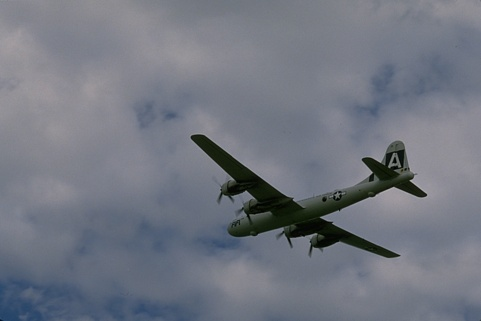
\includegraphics[width=0.49\textwidth]{3096.jpg}
	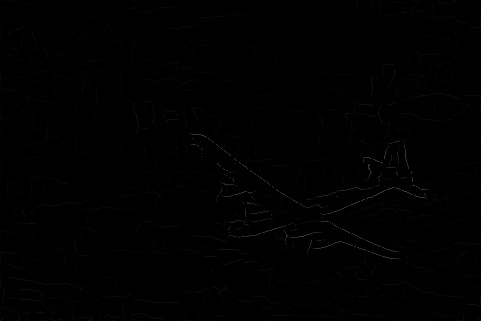
\includegraphics[width=0.49\textwidth]{3096re.jpg}
	\caption{figure 3096 and its result}
\end{figure}

\begin{figure}[H]
	\centering
	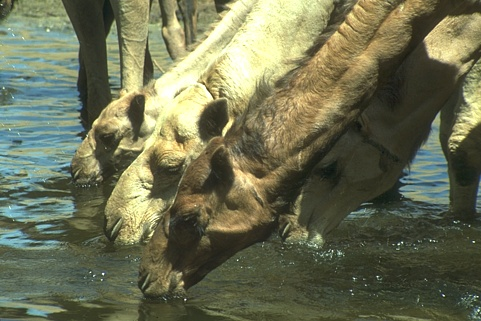
\includegraphics[width=0.49\textwidth]{16077.jpg}
	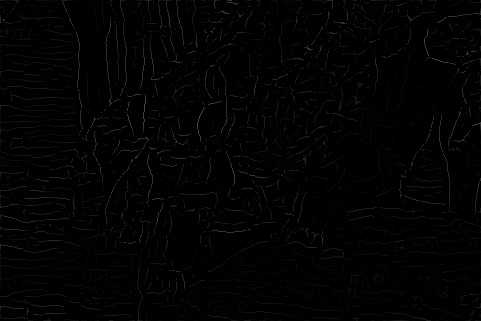
\includegraphics[width=0.49\textwidth]{16077re.jpg}
	\caption{figure 16077 and its result}
\end{figure}

\begin{figure}[H]
	\centering
	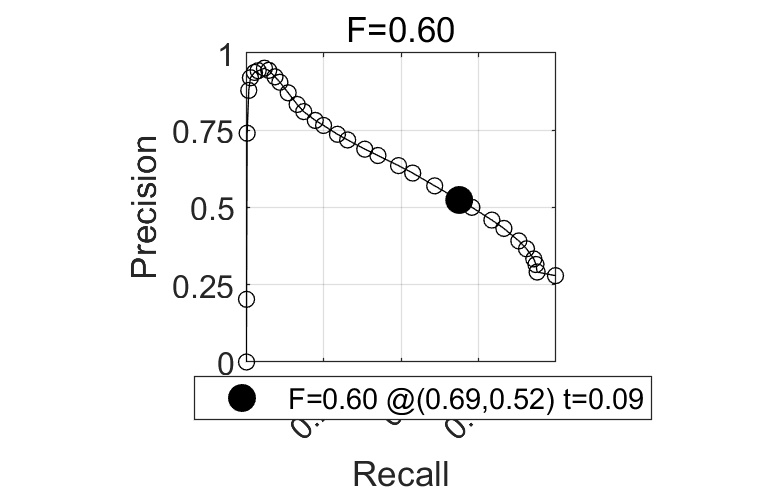
\includegraphics[width=0.49\textwidth]{pr_full.jpg}
	\caption{precision-recall plots}
\end{figure}

Method gradient:	overall F-score = 0.595		average F-score = 0.629

\subsection{question1.2}
The bank of filters I used for part(b) is a set of steerable filters:
$$\{(cos(a)*dGx, sin(a)*dGy)\}$$
for $a=\pi*(i-1)/6,i=1,\cdots,6$, where $(dGx,dGy)$ is the gradient of a Gaussian filter.

\begin{figure}[H]
	\centering
	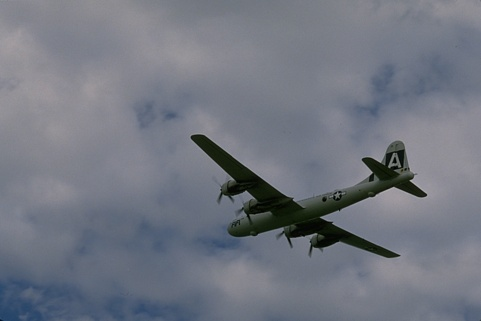
\includegraphics[width=0.49\textwidth]{3096.jpg}
	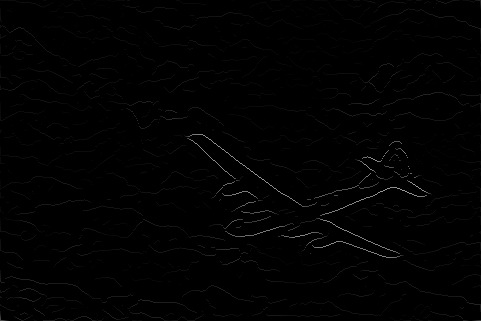
\includegraphics[width=0.49\textwidth]{3096re2.jpg}
	\caption{figure 3096 and its result}
\end{figure}

\begin{figure}[H]
	\centering
	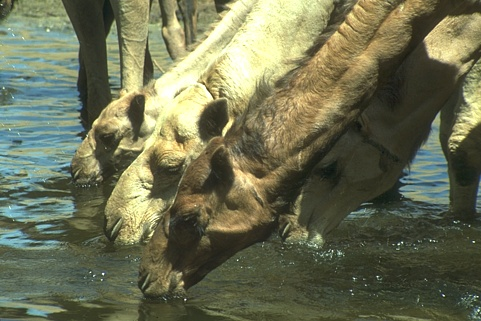
\includegraphics[width=0.49\textwidth]{16077.jpg}
	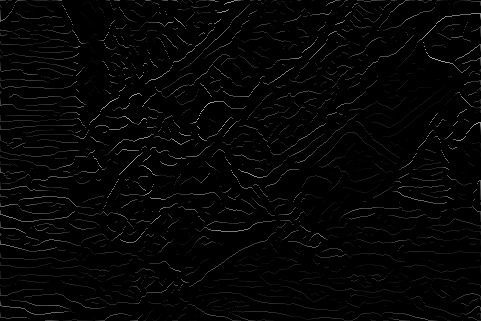
\includegraphics[width=0.49\textwidth]{16077re2.jpg}
	\caption{figure 16077 and its result}
\end{figure}

\begin{figure}[H]
	\centering
	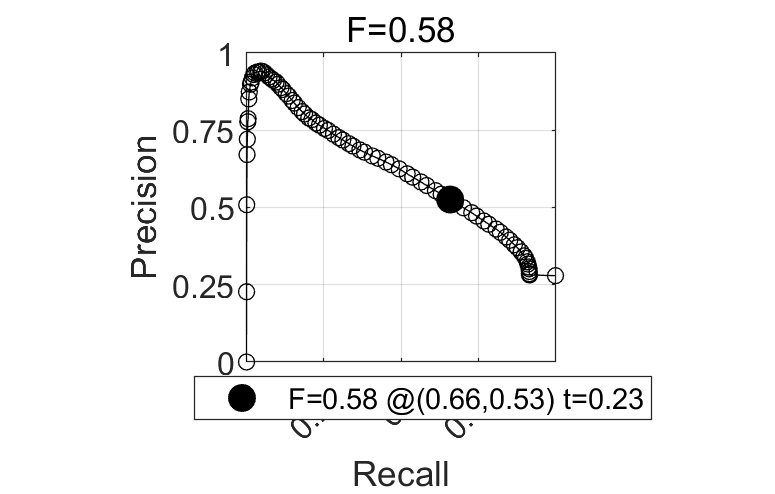
\includegraphics[width=0.49\textwidth]{pr_full2.jpg}
	\caption{precision-recall plots}
\end{figure}

Method oriented:	overall F-score = 0.585, average F-score = 0.624


\subsection{question1.3}
Idea: Use bilateral filters to smooth the image\\
Reason: the Gaussian filters will blur the edges, which may results in bad edge detection; bilateral filters possess the property of "Edge Preseving"
%��bilateral blur �㷨���н��롣Bilateral blur����ڴ�ͳ�ĸ�˹blur��˵����Ҫ��һ�����Լ��ɿ��Ա��ֱ�Ե��Edge Preseving��

\section{Question 2}
\subsection{question2.1}
To implement the function
$$function[labelIm] = quantizeFeats(featIm, meanFeats)$$
we fetch each row pixels of $featIm$, calculate the distances to the $meanFeats$ using 'dist2' function. Then use the index whose distance is the minimal as the label (cluster membership).

\subsection{question2.2}
The function
$$function[textons] = createTextons(imStack, bank, k)$$
computes a texton "codebook" (i.e., set of quantized filter bank responses) based on a sample of filter responses. \\
It iterates through the image stack and filters each image with all filters in the filter bank. Then it samples a subset of the pixels' filter responses and puts it into the dataset "Textons". \\
Now it only need to do k-means clustering on the dataset using 'kmeans' and returns the clusters.

\subsection{question2.3}
In function
$$function[featIm] = extractTextonHists(origIm, bank, textons, winSize)$$
constructs a texton histogram for each pixel based on the frequency of each texton within its neighborhood (as defined by a local window of fixed scale winSize). \\
Specifically, the origin image is filtered by all the filters in the filter bank. Then we get the cluster membership of each pixel to the textons using 'quantizeFeats' that has been implemented earlier:
$$labelIm = quantizeFeats(filteredIm, textons);$$
After that, we only need to get the frequency for the window of each pixel. Here I fetch the window matrix and using 'tabulate' function to obatin the infomation.

\subsection{question2.4}
The function
$$function[colorLabelIm, textureLabelIm] $$$$= compareSegmentations(origIm, bank, textons, winSize, numColorRegions, numTextureRegions)$$
comes in two parts, the first part of which simply does the k-means on the feature space of colors for each pixel. \\
For the second part, we're supposed to extract the texton histogram of the origin image and then do the k-means based on it. Notice that the function 'extractT extonHists' takes in a grayscale image, so we should transform the original RGB image into a grayscale image first:
$$textonHist = extractTextonHists(rgb2gray(origIm), bank, textons, winSize);$$

\subsection{Results and Explanations}
Note: the number of textons is set to be $k\_textons = 17$
\subsubsection{results}
\begin{figure}[H]
	\centering
	\subfloat{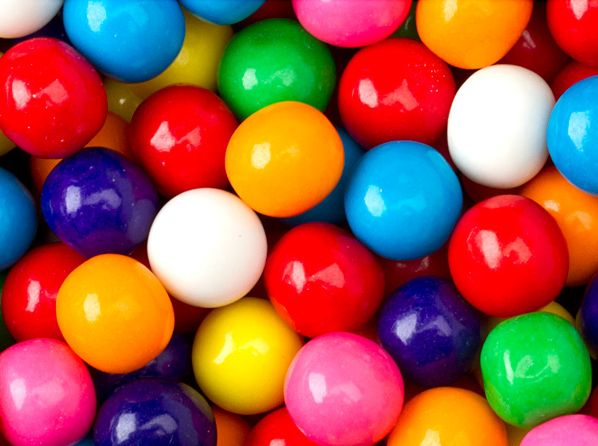
\includegraphics[width=0.35\textwidth]{gumballs.jpg}}
	\newline
	\subfloat{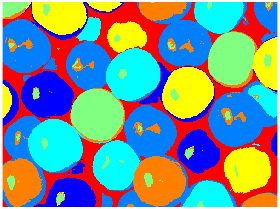
\includegraphics[width=0.35\textwidth]{gumballs1.png}}
	\subfloat{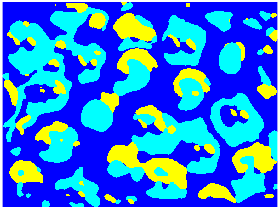
\includegraphics[width=0.35\textwidth]{gumballs2.png}}
	\caption{gumballs.jpg and results, (winSize, numColorRegions, numTextureRegions)=(12, 7, 3)}
\end{figure}

\begin{figure}[H]
	\centering
	\subfloat{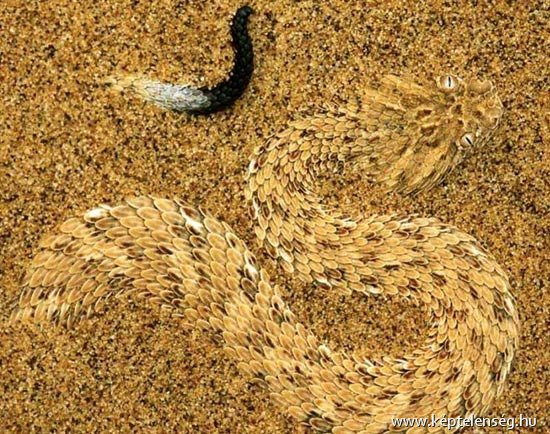
\includegraphics[width=0.35\textwidth]{snake.jpg}}
	\newline
	\subfloat{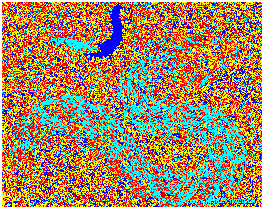
\includegraphics[width=0.35\textwidth]{snake1.png}}
	\subfloat{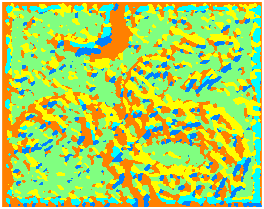
\includegraphics[width=0.35\textwidth]{snake2.png}}
	\caption{snake.jpg and results, (winSize, numColorRegions, numTextureRegions)=(6, 4, 5)}
\end{figure}

\begin{figure}[H]
	\centering
	\subfloat{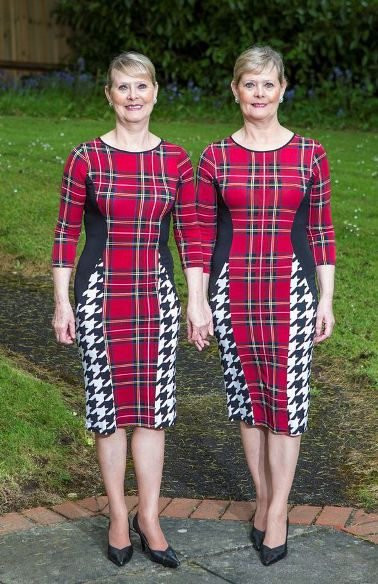
\includegraphics[width=0.22\textwidth]{twins.jpg}}
	\newline
	\subfloat{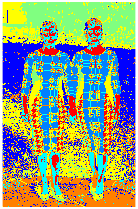
\includegraphics[width=0.22\textwidth]{twins1.png}}
	\subfloat{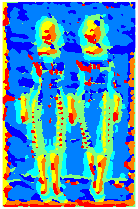
\includegraphics[width=0.22\textwidth]{twins2.png}}
	\caption{twins.jpg and results, (winSize, numColorRegions, numTextureRegions)=(9, 7, 7)}
\end{figure}

\begin{figure}[H]
	\centering
	\subfloat{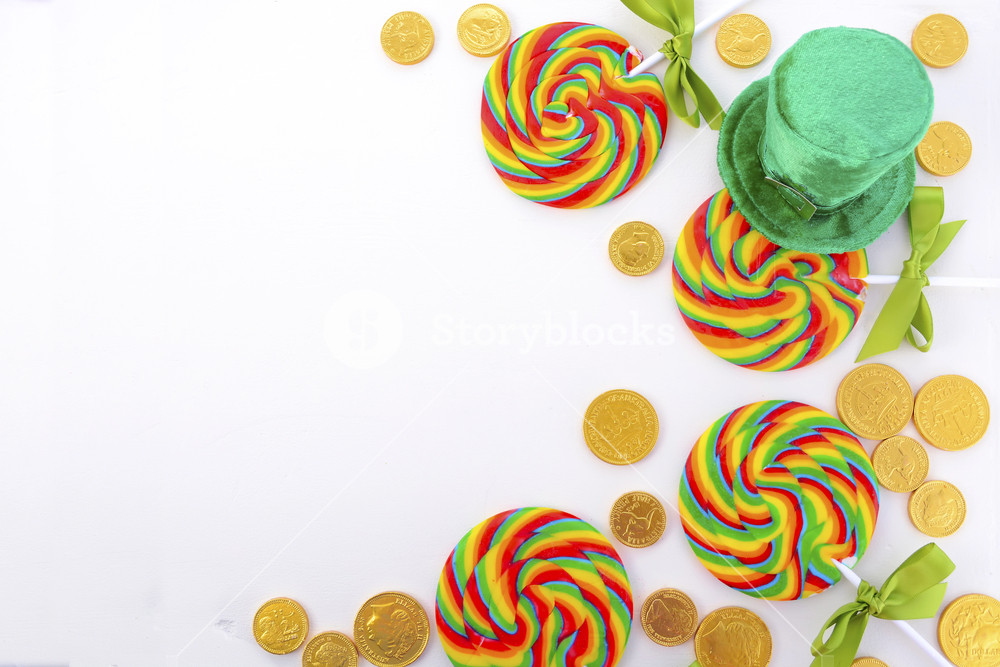
\includegraphics[width=0.35\textwidth]{coins.jpg}}
	\newline
	\subfloat{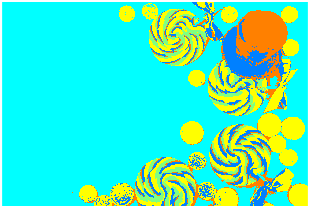
\includegraphics[width=0.35\textwidth]{coins1.png}}
	\subfloat{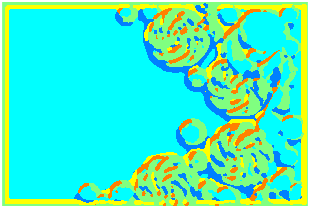
\includegraphics[width=0.35\textwidth]{coins2.png}}
	\caption{coins.jpg and results, (winSize, numColorRegions, numTextureRegions)=(10, 5, 5)}
\end{figure}

\subsubsection{Explanations}
Choose two window sizes for texture representation:
\begin{figure}[H]
	\centering
	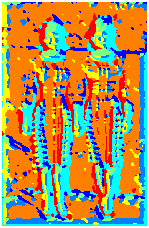
\includegraphics[width=0.25\textwidth]{twins_smallWin.png}
	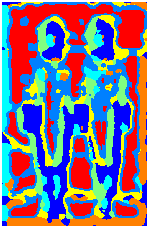
\includegraphics[width=0.25\textwidth]{twins_largeWin.png}
	\caption{two texture segmentation results of twins.jpg, winSize is 5 and 22}
\end{figure}
we can easily find that small window sizes lead to detailed texture while large window sizes lead to less details. (Notice: Larger winSizes were chosen such as 35 and 50, but they didn't lead to convergence in kmeans. )\\% and smoother background.
Run the texture segmentation results with another filter bank which is the subset of the given filter bank. The filter bank contains all the horizontal filters:
$$subbank = bank(:,:,1:6:end);$$
\begin{figure}[H]
	\centering
	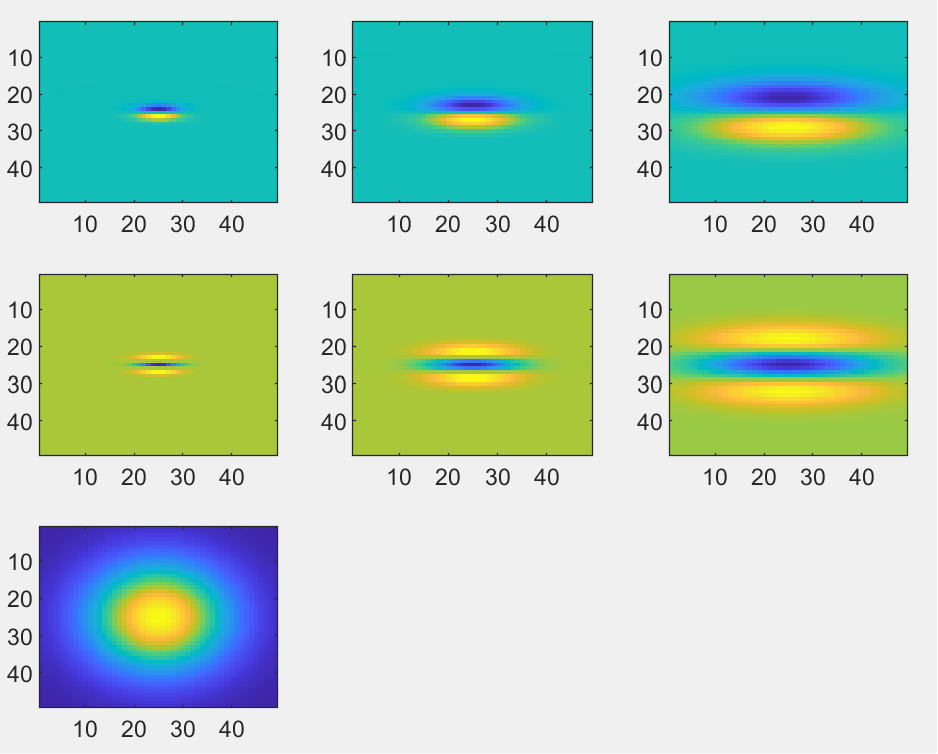
\includegraphics[width=0.49\textwidth]{filter_bank.png}
	\caption{horizontal filter bank}
\end{figure}
We get:
\begin{figure}[H]
	\centering
	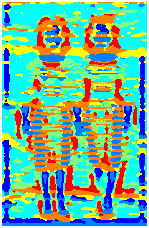
\includegraphics[width=0.25\textwidth]{twins_filter.png}
	\caption{texture segmentation results of twins.jpg, with horizontal filter bank}
\end{figure}
Compared to the previous texture segmentation result, we can find that only horizontal textures are extracted. So we conclude that filters with different orientation are needed for the texture segmentation. 

\bibliographystyle{plain}
\bibliography{ref}
\end{document}